\documentclass[10pt,a4paper]{llncs}

\frontmatter
\usepackage{cmap}

\usepackage[greek,english]{babel}
\languageattribute{greek}{polutoniko}
\usepackage{hyperref}
\addto\extrasenglish{\def\figureautorefname{figure}}
\addto\extrasenglish{\def\subsectionautorefname{section}}
\addto\extrasenglish{\def\subsubsectionautorefname{section}}

\usepackage{amsmath,amssymb}
\usepackage{lmodern}
\usepackage{stmaryrd}
\usepackage{comment}
\usepackage{ifthen}
\usepackage{makeidx}

\usepackage{bussproofs}
\usepackage{graphicx}
\EnableBpAbbreviations
\usepackage{mdframed}
\newenvironment{scprooftree}[1]%
  {\gdef\scalefactor{#1}\begin{center}\proofSkipAmount \leavevmode}%
  {\scalebox{\scalefactor}{\DisplayProof}\proofSkipAmount \end{center} }
\newenvironment{scprooftree*}[1]%
  {\gdef\scalefactor{#1} \leavevmode\hbox\bgroup}%
  {\scalebox{\scalefactor}{\DisplayProof} \egroup}

\usepackage{natbib}
\usepackage{etoolbox}
\usepackage{xstring}
\makeatletter
\patchcmd{\NAT@test}{\else \NAT@nm}{\else \NAT@nmfmt{\NAT@nm}}{}{}

\DeclareRobustCommand\citepos
  {\begingroup
   \let\NAT@nmfmt\NAT@posfmt% ...except with a different name format
   \NAT@swafalse\let\NAT@ctype\z@\NAT@partrue
   \@ifstar{\NAT@fulltrue\NAT@citetp}{\NAT@fullfalse\NAT@citetp}}

\let\NAT@orig@nmfmt\NAT@nmfmt
\def\NAT@posfmt#1{%
  \StrRemoveBraces{#1}[\NAT@temp]%
  \IfEndWith{\NAT@temp}{s}
    {\NAT@orig@nmfmt{#1'}}
    {\NAT@orig@nmfmt{#1's}}}
\makeatother
\newcommand{\mathplus}[0]{+}

% abbrev.
\def\NLIBC{NL$_{\text{IBC}}$}
\def\I{\ensuremath{\mathbf{I}}}
\def\B{\ensuremath{\mathbf{B}}}
\def\C{\ensuremath{\mathbf{C}}}
\def\Q{\ensuremath{\mathbf{Q}}}

% only during writing
\usepackage{xcolor}


\begin{document}

\mainmatter%
\title{Strong and weak quantifiers in focused \NLCL}
%\author{Pepijn Kokke}
%\institute{%
%  Institute for Logic, Language and Computation\\
%  University of Amsterdam, Amsterdam\\
%  \email{pepijn.kokke@gmail.com}}
\maketitle

\begin{abstract}
  We propose an improvement of \citepos{barker2015} {\NLCL} for which
  derivability is decidable, which has a normal-form for proof search,
  can analyse scope islands, and distinguish between strong and weak
  quantifiers.
\end{abstract}

\section{Introduction}\label{sec:introduction}

In \citeyear{kiselyov2014}, \citet{kiselyov2014} published a
paper in which they presented an elegant approach to the anaysis of
various scope-related phenomena using, what they call, the
continuation hierarchy.
The phenomena they cover are scope ambiguity, scope islands and strong
and weak quantifiers.
They cover these phenomena using a mechanism which works on the
sentence's \emph{semantics}, independent of whatever form of grammar
is used.

At around the same time, \citepos{barker2015} published a book
containing their findings on {\NLLAM} and {\NLCL}, a pair of grammar
logics, both with the ability to analyse scope ambiguity using a
strictly \emph{syntactic} mechanism.
In addition, these logics can analyse ``parastic scope''
\citep{barker2007,barker2015} and a quantifiers which change the
result type of the expressions they take scope over.
However, neither of these logics is capable of analysing scope islands
or strong and weak quantifiers.

In this paper, we rework {\NLCL} to a calculus which can analyse both
scope islands and strong and weak quantifiers, without losing
the ability to analyse parasitic scope or changing result types.
For this, we base ourselves on work by \citet{moortgat1996} and
\citet{moortgat2012}. As a bonus, their approach requires a strict
focusing regime. Therefore, adopting it results in the elimination of
spurious ambiguity, and greatly enhances the efficiency of proof
search when compared to \citepos{barker2015} {\NLCL}.

We will start our discussion by giving several examples of each of the
aforementioned phenomena. The following sentences are examples of scope
ambiguity, scope islands and weak quantifiers, respectively. They are
given together with their expected semantics, and are based on
examples by \citet[][p.\ 608, 622]{szabolcsi2000}.
\eenumsentence{\label{ex:scope-ambiguity}
\item[]\hspace*{-0.5\leftmargin}%
  ``Someone read every book.''
\item%
  \(
  \exists{x}.\PERSON(x)\wedge\forall{y}.\BOOK(y)\supset\READ(x,y)
  \)
\item%
  \(
  \forall{y}.\BOOK(y)\supset\exists{x}.\PERSON(x)\wedge\READ(x,y)
  \)}
\eenumsentence{\label{ex:scope-island}
\item[]\hspace*{-0.5\leftmargin}%
  ``Someone said Kurt wrote every book.''
\item%
  \(
  \exists{x}.\PERSON(x)\wedge\SAY(x,\forall{y}.\BOOK(y)\supset\WROTE(\KURT,y))
  \)}
\eenumsentence{\label{ex:weak-quantifier}
\item[]\hspace*{-0.5\leftmargin}%
  ``Everyone said [Kurt dedicated a book to Mary].''
\item%
  \(
  \forall{x}.\PERSON(x)\supset\SAY(x,\exists{y}.\BOOK(y)
  \wedge\DEDICATE(\KURT,\MARY,y))
  \)
\item%
  \(
  \forall{x}.\PERSON(x)\supset\exists{y}.\BOOK(y)
  \wedge\SAY(x,\DEDICATE(\KURT,\MARY,y))
  \)
\item%
  \(
  \exists{y}.\BOOK(y)
  \wedge\forall{x}.\PERSON(x)\supset\SAY(x,\DEDICATE(\KURT,\MARY,y))
  \)}
The first of these examples is a canonical example of scope
ambiguity.
%
Example (\ref{ex:scope-island}) demonstrates a scope
island: there is no reading in which ``every book'' scopes out of the
embedded clause, as this reading would imply that the speaker made a
separate speech act for every book: ``Kurt wrote
Slaughterhouse-Five'', ``Kurt wrote Cat's Cradle'', ``Kurt
wrote\ldots''
%
Finally, example (\ref{ex:weak-quantifier}) shows that
indefinites \emph{can} scope out of scope islands.

We add two more sentences, which are examples of a quantifier which
changes the result type, and of parasitic scope, respectively. These
examples based on those given by \citepos[][p.\ 208]{barker2015} and
\citet{kiselyov2015b}.
\eenumsentence{\label{ex:changing-result-type}
\item[]\hspace*{-0.5\leftmargin}%
  ``John read a book [the author of which] feared the ocean.''
\item%
  \(
  \exists{x}.\BOOK(x)
  \wedge\FEAR(\iota(\lambda{y}.\OF(y,\AUTHOR,x)),\iota(\OCEAN))
  \wedge\READ(\JOHN,x)
  \)}
\eenumsentence{\label{ex:parasitic-scope}
\item[]\hspace*{-0.5\leftmargin}%
  ``Everyone feared the same ocean.''
\item%
  \(
  \exists{z}.\forall{y}.\FEAR(y,\iota(\lambda{x}.\OCEAN(x)\wedge{x=z}))
  \)}
These last two examples will play a less important role, as {\NLCL} is
already capable of analysing both. However, in order to demonstrate
that we have not lost that capability, we will provide analyses of
both near the end of this paper.

\section{Background}
In this section, we will briefly discuss {\NLCL} and its sibling,
{\NLLAM}. {\NLCL} is an extension to the non-associative Lambek
calculus \citep[NL;][]{lambek1961}.
The history behind {\NLCL} is somewhat intricate, but helpful to
understanding, so we will briefly go over it.
The initial idea comes from the practice of encoding quantifier
movement as a tree transformation which introduces a
binder~\citep{heim1998}:
\begin{center}
  \begin{minipage}{0.4\linewidth}\centering
    \begin{tikzpicture}
      \tikzset{level distance=4ex}
      \tikzset{sibling distance=0pt}
      \Tree [ john [ likes everyone ] ]
    \end{tikzpicture}
  \end{minipage}%
  \begin{minipage}{0.05\linewidth}\centering
    $\longleftrightarrow$
  \end{minipage}%
  \begin{minipage}{0.5\linewidth}\centering
    \begin{tikzpicture}
      \tikzset{level distance=4ex}
      \tikzset{sibling distance=0pt}
      \Tree [ everyone [ $\lambda x.$ [ john [ likes $x$ ] ] ] ]
    \end{tikzpicture}
  \end{minipage}
\end{center}
To implement this idea in type-logical grammar,
\citeauthor{barker2015} add a structural $\lambda$-construct to NL,
and added the following structural postulate:\footnote{%
  It is important to note that this construct is \emph{purely
  structural}, and that it is not accompanied by some implicit form of
  computation (e.g.\ $\beta,\eta$-conversions).
}
\begin{align}
  \tag{$\lambda$}
  \Sigma[\Gamma] \longleftrightarrow \Gamma\hprod\lambda{x}.\Sigma[x]
  \label{eqn:lambda}
\end{align}
As can be seen, the~\eqref{eqn:lambda} postulate uses a new
connective: the $\hprod$ (hollow product).
This connective is part of a new residuated family $\{\himpr, \hprod,
\himpl\}$, which starts out as a copy of $\{\impr, \prod,
\impl\}$.
However, the addition of the~\eqref{eqn:lambda} postulate allows you
to raise any constituent to the top-left position in the structure,
where---if it has the right type---it can be ``resolved'' against the
top-level type as follows:
\begin{scprooftree}
  \AXC{$\Sigma[{A}]\fCenter{B}$}
  \RightLabel{\eqref{eqn:lambda}}
  \UIC{${A}\hprod\lambda{x}.\Sigma[x]\fCenter{B}$}
  \RightLabel{R$\himpr$}
  \UIC{$\lambda{x}.\Sigma[x]\fCenter{A\himpr B}$}
  \AXC{${C}\fCenter{D}$} \RightLabel{L$\himpl$}
  \BIC{${C\himpl(A\himpr B)}\hprod\lambda{x}.\Sigma[x]\fCenter{D}$}
  \RightLabel{\eqref{eqn:lambda}}
  \UIC{$\Sigma[{C\himpl(A\himpr B)}]\fCenter{D}$}
\end{scprooftree}
\citeauthor{barker2015} call resulting system {\NLLAM}.
While {\NLLAM} fulfils the promise of allowing a syntactic analysis of
quantifier raising, scope ambiguity and parasitic scope, it has some
problems.
Most notably, the system is hard to formalise and to reason about,
largely due to the presence of a binding construct in the syntax of
structures.
While it is not impossible to formalise, the~\eqref{eqn:lambda}
postulate greatly complicates meta-logical proofs.

To address this issue, and to ease their own investigation of the
formal properties of {\NLLAM}, \citet[][ch.\ 17]{barker2015} introduce
{\NLCL}.
This system uses the fact that $\lambda$-terms can be represented as
combinators in combinatory logic, which removes the need for a binding
construct.
\citeauthor{barker2015} use a variant of Sch\"onfinkel's mapping to
encode the \emph{linear} $\lambda$-construct as applications of the
combinators $\I$, $\B$ and $\C$:\footnote{%
  One can easily verify that the $\lambda$-construct introduced
  by~\eqref{eqn:lambda} is linear.
}\footnote{%
  When comparing these equations to the \I\B\C-rules in
  \autoref{fig:nlcl}, note that $\prod$ encodes function application,
  but $\hprod$ encodes \emph{flipped} function application.
}
\[
  \I x     = x,
  \qquad
  \B x y z = x (y z),
  \qquad
  \C x y z = x  z y
\]
The resulting system is presented in \autoref{fig:nlcl}.\footnote{%
  In \autoref{fig:nlcl}, and for the remainder of this paper, the
  letters $\Gamma$ and $\Delta$ are reserved for structures, whereas
  the $\Sigma$ is used for contexts.
}

\begin{figure}[h!]
  \centering

  \begin{scprooftree*}
    \AXC{}\RightLabel{Ax}\UIC{$A\fCenter A$}
  \end{scprooftree*}

  \vspace*{1\baselineskip}
  \begin{scprooftree*}
    \AXC{$\Gamma\fCenter A$}
    \AXC{$\Sigma[B]\fCenter C$}
    \RightLabel{$\impr L$}
    \BIC{$\Sigma[\Gamma\prod A\impr B]\fCenter C$}
  \end{scprooftree*}%
  \begin{scprooftree*}
    \AXC{$A\prod\Gamma\fCenter B$}
    \RightLabel{$\impr R$}
    \UIC{$\Gamma\fCenter A\impr B$}
  \end{scprooftree*}%
  \begin{scprooftree*}
    \AXC{$\Gamma\fCenter A$}
    \AXC{$\Sigma[B]\fCenter C$}
    \RightLabel{$\impl L$}
    \BIC{$\Sigma[B\impl A \prod\Gamma]\fCenter C$}
  \end{scprooftree*}%
  \begin{scprooftree*}
    \AXC{$\Gamma\prod A\fCenter B$}
    \RightLabel{$\impl R$}
    \UIC{$\Gamma\fCenter B\impl A$}
  \end{scprooftree*}

  \vspace*{1\baselineskip}
  \begin{scprooftree*}
    \AXC{$\Gamma\fCenter A$}
    \AXC{$\Sigma[B]\fCenter C$}
    \RightLabel{$\himpr L$}
    \BIC{$\Sigma[\Gamma\hprod A\himpr B]\fCenter C$}
  \end{scprooftree*}%
  \begin{scprooftree*}
    \AXC{$A\hprod\Gamma\fCenter B$}
    \RightLabel{$\himpr R$}
    \UIC{$\Gamma\fCenter A\himpr B$}
  \end{scprooftree*}%
  \begin{scprooftree*}
    \AXC{$\Gamma\fCenter A$}
    \AXC{$\Sigma[B]\fCenter C$}
    \RightLabel{$\himpl L$}
    \BIC{$\Sigma[B\himpl A \hprod\Gamma]\fCenter C$}
  \end{scprooftree*}%
  \begin{scprooftree*}
    \AXC{$\Gamma\hprod A\fCenter B$}
    \RightLabel{$\himpl R$}
    \UIC{$\Gamma\fCenter B\himpl A$}
  \end{scprooftree*}

  \vspace*{1\baselineskip}
  \begin{scprooftree*}
    \AXC{$\Sigma[A]\fCenter B$}
    \doubleLine\RightLabel{\I}
    \UIC{$\Sigma[A\hprod \I]\fCenter B$}
  \end{scprooftree*}%
  \begin{scprooftree*}
    \AXC{$\Sigma[A\prod(B\hprod C)]\fCenter D$}
    \doubleLine\RightLabel{\B}
    \UIC{$\Sigma[B\hprod((\B\prod A)\prod C)]\fCenter D$}
  \end{scprooftree*}%
  \begin{scprooftree*}
    \AXC{$\Sigma[(A\hprod B)\prod C]\fCenter D$}
    \doubleLine\RightLabel{\C}
    \UIC{$\Sigma[A\hprod((\C\prod B)\prod C)]\fCenter D$}
  \end{scprooftree*}

  \caption{\NLCL\ as presented by \citet{barker2015}.}
  \label{fig:nlcl}
\end{figure}
%%% Local Variables:
%%% mode: latex
%%% TeX-master: "main"
%%% End:


Using the system in \autoref{fig:nlcl}, we can do quantifier raising
in much the same way as we did with the~\eqref{eqn:lambda}
postulate---although, as we now have to raise the quantifier one step
at a time, the proofs are much longer:
\begin{scprooftree}
  \AXC{$\vdots$}\noLine%
  \UIC{$\textsc{john}\prod\textsc{likes}\prod{np}\fCenter{s}$}
  \RightLabel{\I}
  \UIC{$\textsc{john}\prod\textsc{likes}\prod{np}\hprod\I\fCenter{s}$}
  \RightLabel{\B}
  \UIC{$\textsc{john}\prod{np}\hprod{(\B\prod\textsc{likes})\prod\I}\fCenter{s}$}
  \RightLabel{\B}
  \UIC{${np}\hprod(\B\prod\textsc{john})\prod{(\B\prod\textsc{likes})\prod\I}\fCenter{s}$}
  \RightLabel{$\himpr R$}
  \UIC{$(\B\prod\textsc{john})\prod{(\B\prod\textsc{likes})\prod\I}\fCenter{np}\himpr{s}$}
  \AXC{${s}\fCenter{s}$}
  \RightLabel{$\himpl L$}
  \BIC{$\textsc{everyone}\hprod(\B\prod\textsc{john})\prod{(\B\prod\textsc{likes})\prod\I}\fCenter{s}$}
  \RightLabel{\B}
  \UIC{$\textsc{john}\prod{\textsc{everyone}}\hprod{(\B\prod\textsc{likes})\prod\I}\fCenter{s}$}
  \RightLabel{\B}
  \UIC{$\textsc{john}\prod\textsc{likes}\prod{\textsc{everyone}\hprod\I}\fCenter{s}$}
  \RightLabel{\I}
  \UIC{$\textsc{john}\prod\textsc{likes}\prod{\textsc{everyone}}\fCenter{s}$}
\end{scprooftree}
The labels \textsc{john}, \textsc{likes} and \textsc{everyone}
abbreviate the types ${np}$, $({np}\impr{s})\impl{np}$ and
${s}\himpl({np}\himpr{s})$, respectively. For a more detailed account
of the relation between {\NLLAM} and {\NLCL}, see \citet{barker2015}.
For a more detailed account of various encodings of combinatorial
logic in structural rules, amongst which the encoding of the linear
lambda construct used by \citeauthor{barker2015}, see
\citet{finger2001}.


\section{Scope islands for {\NLCL}}
\label{sec:scope-islands}

Our aim for this section is to present an extension to {\NLCL} which
will allow us to analyse scope islands, and therefore example
(\ref{ex:scope-island}).

To analyse scope islands, we need some way to block quantifier
movement. If you look at the \I\B\C-rules in \autoref{fig:nlcl}, you
will notice that they allow constituents attached to (the left of) a
hollow product to move past solid products.
This leads us to suggest a fairly simple solution:
insert \emph{anything} that is not solid product.
For this, we use a residuated pair of unary connectives, $\di$ and
$\sq$~\citep{morrill1994,moortgat1996}.
The relevant rules are presented in \autoref{fig:scope-islands}.

\begin{figure}[h!]
  \centering

  \begin{scprooftree*}
    \AXC{$\Sigma[A]\fCenter B$}
    \RightLabel{$\sq L$}
    \UIC{$\Sigma[{\di[\sq A]}]\fCenter B$}
  \end{scprooftree*}%
  \begin{scprooftree*}
    \AXC{$\di[\Gamma]\fCenter B$}
    \RightLabel{$\sq R$}
    \UIC{$\Gamma\fCenter\sq B$}
  \end{scprooftree*}%
  \begin{scprooftree*}
    \AXC{$\Sigma[{\di[A]}]\fCenter B$}
    \RightLabel{$\di L$}
    \UIC{$\Sigma[{\di A }]\fCenter B$}
  \end{scprooftree*}%
  \begin{scprooftree*}
    \AXC{$\Gamma\fCenter B$}
    \RightLabel{$\di R$}
    \UIC{$\di[\Gamma]\fCenter\di B$}
  \end{scprooftree*}

  \caption{Scope islands for \NLCL.}
  \label{fig:scope-islands}
\end{figure}
%%% Local Variables:
%%% mode: latex
%%% TeX-master: "main"
%%% End:


\noindent
Using these connectives, we can assign `said' the type
$({np}\impr{s})\impl\di{s}$. Instead of taking a sentence-argument
from the right, `said' now takes a \emph{closed-off} sentence---a
scope island. Have a look at the derivation for example
(\ref{ex:scope-island}) given below:
\begin{scprooftree}
  \AXC{$\vdots$}\noLine%
  \UIC{$\textsc{Kurt}\prod\textsc{wrote}\prod\textsc{every}
    \prod\textsc{book}\fCenter{s}$}
  \RightLabel{$\di R$}
  \UIC{$\langle \textsc{Kurt}\prod\textsc{wrote}\prod
    \textsc{every}\prod\textsc{book}\rangle \fCenter\di{s}$}
  \AXC{$\vdots$}\noLine%
  \UIC{$\textsc{someone}\prod{({np}\impr{s})}\fCenter{s}$}
  \RightLabel{$\impl L$}
  \BIC{$\textsc{someone}\prod\textsc{said}\prod\langle
    \textsc{Kurt}\prod\textsc{wrote}\prod\textsc{every}\prod
    \textsc{book}\rangle\fCenter{s}$}
\end{scprooftree}
As long as the scope island (written $\di[\cdot]$) is in place,
`$\textsc{every}\prod\textsc{book}$' cannot be raised past it, for
there is no rule which allows anything to move past a diamond.
But in order to remove the scope island, it has to be eliminated
against the $\di{s}$ argument of `said', and doing so isolates the
embedded clause in its own branch of the proof.\footnote{%
  The presence of the structural diamond in the endsequent
  may seem problematic, but recall that from the perspective of
  backward-chaining search we assign semantics to a \emph{known}
  sentence structure. If we switch to forward-chaining search, i.e.\ %
  to parsing, the need for a scope island will be inferred from the
  type of `said'.
}

\section{Strong and weak quantifiers}
\label{sec:strong-and-weak}

In the previous section, we presented an extension to {\NLCL} which
enabled us to analyse scope islands.
This extension blocks all quantifier movement out of scope islands.
Example (\ref{ex:weak-quantifier}) demonstrates that this is too coarse
an approach.
Specifically, we would like to allow weak quantifiers, such as
indefinites, to scope out of scope islands.

We could approach this issue as a syntactic problem, and encode it
using structural rules, as we did with quantifier movement and scope
islands.\footnote{%
  For instance, we could split the family $\himpr, \hprod, \himpl$
  into two separate families, $\himpr^w, \hprod^w, \himpl^w$ and
  $\himpr^s, \hprod^s, \himpl^s$, each with their own copies of the
  \I\B\C-rules, and add a structural rule which selectively allows
  weak quantifiers to move past scope islands.}
However, \citet{szabolcsi2000} writes that ``indefinites acquire their
existential scope in a manner that does not involve movement and is
essentially syntactically unconstrained.''
Therefore, we feel that a syntactic approach would be out of place.

How do we approach the problem of weak quantifiers as a semantic
problem? The solution is to use continuation-passing style (CPS).
But how? Early attempts, such as the work by \citep{barker2002},
often works by applying a CPS translation directly to the semantic
terms. Such approaches, however, face a fundamental dilemma.
Because the CPS translation is applied to a solitary semantic term,
a deterministic translation cannot introduce scope ambiguity---or any
ambiguity, for that matter.
However, making the CPS translation sufficiently nondeterministic
without causing spurious ambiguity is an arduous task. When
\citeauthor{barker2002} makes the translation ambiguous, in order to
capture scope ambiguity, this leads to the number of introduced
ambigous interpretations growing exponentially with the sentence
length.
More recent approaches, such as the work by \citet{kiselyov2014}, are
much more sophisticated. Their approach allows for the creation of
quantifiers of different strengths (e.g.\ $\text{everyone}_1$,
$\text{everyone}_2$, \dots) essentially reducing scope ambiguity
to lexical ambiguity. As a linguistic standpoint, this feels wrong.
Furthermore, their framework was engineered to be able to analyse
phenomena such as scope islands and weak quantifiers.
This makes it too expressive (and intricate) for the task at hand.

Instead, we base our CPS semantics on the approach of
\citet{moortgat2012} and \citet{bastenhof2013}, who manage to
elegantly integrate CPS semantics into their grammar logic.
\citeauthor{moortgat2012} set up a calculus which enforces
one crucial property: every proof in the grammar logic is associated
with \emph{unique, normal-form semantics}.
In the context of scope ambiguity, this means that each way to
interpret a sentence with ambiguous scope corresponds to exactly one
proof in the grammar logic.

\subsubsection{Focused {\NLCL}}%
\label{sec:normal-form}

\citet[][sec. 3.1]{moortgat2012} define a normal-form calculus for the
Lambek-Grishin calculus (LG).
They refer to this calculus as fLG---for \emph{focused} LG, after
the technique, pioneered by \citet{andreoli2001}, which
they use in their calculus.
As NL is a fragment of LG, we can trivially extract a normal-form
calculus for NL from their work.
We will, in their style, refer to this calculus as fNL.

It is important to note that they develop their calculus within the
framework of display calculus \citep{belnap1982}.
One advantage of this framework is that we can freely add structural
rules, without fear that we will lose the cut-elimination property.
\citepos{barker2015} extension of NL, {\NLCL}, consists solely of a copy
of an existing modality ($\himpr,\hprod,\himpl$) and a number of
structural rules.
Therefore, by applying these same changes, we can extend fNL to focsed
{\NLCL}---or {f\NLCL}.
The result is presented in \autoref{fig:focused-nlcl},
together with the focused version of the extension for scope islands
from \autoref{sec:scope-islands}.

\begin{figure}[b]
  \centering
  \scalebox{\defscalefactor}{\(\!
    \begin{aligned}
      &\text{Atom } \alpha &&::= {s}\mid{n}\mid{np}\mid\ldots\\
      &\text{Type } A, B   &&::= {\alpha}\mid{A\impr B}\mid{B\impl A}
      \mid{A\himpr B}\mid{B\himpl A}\mid{\di A}\mid{\sq A}\\
      &\text{Struct$^-$ } \Delta &&::= \st{A}\mid
      {\Gamma\impr\Delta}\mid{\Delta\impl\Gamma}\mid
      {\Gamma\himpr\Delta}\mid{\Delta\himpl\Gamma}\mid{\sq[\Delta]}\\
      &\text{Struct$^+$ } \Gamma &&::=
      \st{A}\mid{\Gamma_1\prod\Gamma_2}\mid{\Gamma_1\hprod\Gamma_2}\mid
      \I\mid\B\mid\C\mid{\di[\Gamma]}\\
      &\text{Context } \Sigma &&::=
      \Box\mid{\Sigma\prod\Gamma}\mid{\Gamma\prod\Sigma}
    \end{aligned}
  \)}

  \vspace*{1\baselineskip}
  \scalebox{\defscalefactor}{\(\!
    \text{Pol}(s) = -,
    \qquad
    \text{Pol}(n) = +,
    \qquad
    \text{Pol}(np) = +,
    \qquad
    \ldots
  \)}

  \vspace*{1\baselineskip}
  \scalebox{\defscalefactor}{\(\!
    \text{if}\ \text{Pol}(\alpha) = {-}
    \left\lbrace
      \quad
      \begin{aligned}
        \AXC{}
        \RightLabel{Ax$^L$}
        \UIC{$\fc{\alpha}\fCenter\st{\alpha}$}
        \DisplayProof
      \end{aligned}
      \quad
      \middle\vert
      \quad
      \begin{aligned}
        \AXC{}
        \RightLabel{Ax$^R$}
        \UIC{$\st{\alpha}\fCenter\fc{\alpha}$}
        \DisplayProof
      \end{aligned}
      \quad
    \right\rbrace
    \text{if}\ \text{Pol}(\alpha) = {+}
  \)}

  \vspace*{1\baselineskip}
  \scalebox{\defscalefactor}{\(\!
    \text{if}\ \text{Pol}(A) = {-}
    \left\lbrace
      \quad
      \begin{aligned}
        \AXC{$\fc{A}\fCenter\Delta$}
        \RightLabel{Foc$^L$}
        \UIC{$\st{A}\fCenter\Delta$}
        \DisplayProof
        \\[1\baselineskip]
        \AXC{$\Gamma\fCenter\st{A}$}
        \RightLabel{Unf$^R$}
        \UIC{$\Gamma\fCenter\fc{A}$}
        \DisplayProof
      \end{aligned}
      \quad
      \middle\vert
      \quad
      \begin{aligned}
        \AXC{$\Gamma\fCenter\fc{A}$}
        \RightLabel{Foc$^R$}
        \UIC{$\Gamma\fCenter\st{A}$}
        \DisplayProof
        \\[1\baselineskip]
        \AXC{$\st{A}\fCenter\Delta$}
        \RightLabel{Unf$^L$}
        \UIC{$\fc{A}\fCenter\Delta$}
        \DisplayProof
      \end{aligned}
      \quad
    \right\rbrace
    \text{if}\ \text{Pol}(A) = {+}
  \)}

  \vspace*{1\baselineskip}
  \begin{scprooftree*}
    \AXC{$\Gamma\fCenter\fc{A}$}
    \AXC{$\fc{B}\fCenter \Delta$}
    \RightLabel{$\impr L$}
    \BIC{$\fc{A\impr B}\fCenter\Gamma\impr\Delta$}
  \end{scprooftree*}%
  \begin{scprooftree*}
    \AXC{$\Gamma\fCenter\st{A}\impr\st{B}$}
    \RightLabel{$\impr R$}
    \UIC{$\Gamma\fCenter\st{A\impr B}$}
  \end{scprooftree*}%
  \begin{scprooftree*}
    \AXC{$\Gamma\fCenter\fc{A}$}
    \AXC{$\fc{B}\fCenter\Delta$}
    \RightLabel{$\impl L$}
    \BIC{$\fc{B\impl A}\fCenter \Delta\impl\Gamma$}
  \end{scprooftree*}%
  \begin{scprooftree*}
    \AXC{$\Gamma\fCenter\st{B}\impl\st{A}$}
    \RightLabel{$\impl R$}
    \UIC{$\Gamma\fCenter\st{B\impl A}$}
  \end{scprooftree*}

  \vspace*{1\baselineskip}
  \begin{scprooftree*}
    \AXC{$\Gamma\fCenter\fc{A}$}
    \AXC{$\fc{B}\fCenter \Delta$}
    \RightLabel{$\himpr L$}
    \BIC{$\fc{A\himpr B}\fCenter\Gamma\himpr\Delta$}
  \end{scprooftree*}%
  \begin{scprooftree*}
    \AXC{$\Gamma\fCenter\st{A}\himpr\st{B}$}
    \RightLabel{$\himpr R$}
    \UIC{$\Gamma\fCenter\st{A\himpr B}$}
  \end{scprooftree*}%
  \begin{scprooftree*}
    \AXC{$\Gamma\fCenter\fc{A}$}
    \AXC{$\fc{B}\fCenter\Delta$}
    \RightLabel{$\himpl L$}
    \BIC{$\fc{B\himpl A}\fCenter\Delta\himpl\Gamma$}
  \end{scprooftree*}%
  \begin{scprooftree*}
    \AXC{$\Gamma\fCenter\st{B}\himpl\st{A}$}
    \RightLabel{$\himpl R$}
    \UIC{$\Gamma\fCenter\st{B\himpl A}$}
  \end{scprooftree*}

  \vspace*{1\baselineskip}
  \begin{scprooftree*}
    \AXC{$\Gamma_2\fCenter\Gamma_1\impr\Delta$}
    \doubleLine\RightLabel{Res$\impr\prod$}
    \UIC{$\Gamma_1\prod\Gamma_2\fCenter\Delta$}
  \end{scprooftree*}%
  \begin{scprooftree*}
    \AXC{$\Gamma_1\fCenter\Delta\impl\Gamma_2$}
    \doubleLine\RightLabel{Res$\impl\prod$}
    \UIC{$\Gamma_1\prod\Gamma_2\fCenter\Delta$}
  \end{scprooftree*}%
  \begin{scprooftree*}
    \AXC{$\Gamma_2\fCenter\Gamma_1\himpr\Delta$}
    \doubleLine\RightLabel{Res$\himpr\hprod$}
    \UIC{$\Gamma_1\hprod\Gamma_2\fCenter\Delta$}
  \end{scprooftree*}%
  \begin{scprooftree*}
    \AXC{$\Gamma_1\fCenter\Delta\himpl\Gamma_2$}
    \doubleLine\RightLabel{Res$\himpl\hprod$}
    \UIC{$\Gamma_1\hprod\Gamma_2\fCenter\Delta$}
  \end{scprooftree*}

  \vspace*{1\baselineskip}
  \begin{scprooftree*}
    \AXC{$\Gamma\fCenter\Delta$}
    \doubleLine\RightLabel{$\I$}
    \UIC{$\Gamma\hprod\I\fCenter\Delta$}
  \end{scprooftree*}
  \begin{scprooftree*}
    \AXC{$\Gamma_1\prod(\Gamma_2\hprod\Gamma_3)\fCenter\Delta$}
    \doubleLine\RightLabel{$\B$}
    \UIC{$\Gamma_2\hprod((\B\prod\Gamma_1)\prod\Gamma_3)\fCenter\Delta$}
  \end{scprooftree*}
  \begin{scprooftree*}
    \AXC{$(\Gamma_1\hprod\Gamma_2)\prod\Gamma_3\fCenter\Delta$}
    \doubleLine\RightLabel{$\C$}
    \UIC{$\Gamma_1\hprod((\C\prod\Gamma_2)\prod\Gamma_3)\fCenter\Delta$}
  \end{scprooftree*}

  \vspace*{1\baselineskip}
  \begin{scprooftree*}
    \AXC{$\di[\st{A}]\fCenter\Delta$}
    \RightLabel{$\di L$}
    \UIC{$\st{\di A}\fCenter\Delta$}
  \end{scprooftree*}%
  \begin{scprooftree*}
    \AXC{$\Gamma\fCenter\fc{B}$}
    \RightLabel{$\di R$}
    \UIC{$\di[\Gamma]\fCenter\fc{\di B}$}
  \end{scprooftree*}%
  \begin{scprooftree*}
    \AXC{$\fc{A}\fCenter\Delta$}
    \RightLabel{$\sq L$}
    \UIC{$\fc{\sq A}\fCenter\sq[\Delta]$}
  \end{scprooftree*}%
  \begin{scprooftree*}
    \AXC{$\Gamma\fCenter\sq[\st{B}]$}
    \RightLabel{$\sq R$}
    \UIC{$\Gamma\fCenter\st{\sq B}$}
  \end{scprooftree*}%
  \begin{scprooftree*}
    \AXC{$\Gamma\fCenter[\Delta]$}
    \doubleLine\RightLabel{Res$\sq\di$}
    \UIC{$\di[\Gamma]\fCenter\Delta$}
  \end{scprooftree*}

  \caption{{\NLCL} reworked as a focused display calculus.}
  \label{fig:focused-nlcl}
\end{figure}
%%% Local Variables:
%%% mode: latex
%%% TeX-master: "main"
%%% End:


Equivalence between {f\NLCL} and {\NLCL} can likely be proven using
an intermediate system: display {\NLCL}. One can trivially obtain this
system from the focused system in \autoref{fig:focused-nlcl} by
dropping the focus marker ``$\,\fc{\phantom{\cdot}}\,$'' and the
focusing and unfocusing rules.
Equivalence between the display and focused variants of a system was
proven for classical NL by \citet{bastenhof2011}.
This proof can likely be adapted for {\NLCL}.

% TODO: add reference for proof of equivalence between display NLCL
% and the sequent calculus of NLCL

However, it is important to realise that, even in the absence of a
formal proof of equivalence between {\NLCL} and {f\NLCL}, the second
remains a logical system which can analyse all phenomena which
\citet{barker2015} show {\NLCL} can analyse.\footnote{%
  Throughout the remainder of the paper, whenever we discuss one of
  the phenomena discussed in \autoref{sec:introduction}, we will give
  an example proof in {f\NLCL}. In this way, by the end of this paper,
  this claim will be backed up by evidence.
}

\subsubsection{Decidable proof search}%
\label{sec:decidable-proof-search}

At this point, {f\NLCL} still has a problem, which it shares with
{\NLCL}: it does not have decidable proof search.
Since it is a grammar logic, this means that \emph{parsing} is not
decidable.
The cause of this is the \I-rule, which does not obey the substructure
property.\footnote{%
  In the case of {\NLCL}, this is the subformula property.
}

Admittedly, there are other rules which do not obey the substructure
property: the residuation rules and the {\B} and {\C} rules do not
enjoy it.
However, the residuation rules still enjoy a weak form this property:
they \emph{do not increase} the size of the structure.
This means that we can use loop checking to filter out problematic
branches of the search.
%
More interestingly, the {\B} and {\C} rules have the property that
``whatever goes up, must come down.'' At some point, the quantifier
will reach the top of the expression, and at that point, there are
only two things to do:
\begin{enumerate*}[label= (\arabic*)]
\item resolve the quantifier against the top-level type, thereby
  \emph{eliminating} a connective and breaking out of any loop; or
\item go back down along the same path.
\end{enumerate*}
Yet when searching for a proof with the \I-rule, we can always
introduce another \I.

We will address this issue by restricting access to the \I-rule using
a license.
This license will be a new unary connective, written $\q{A}$.
Semantically, this logical connective corresponds to a hollow product
with a right-hand {\I} (i.e.\ ${A}\hprod\I$).
However, as we want neither hollow products, nor the unit $\I$, on the
logical level, we capture these in a single connective.
We remove the $\I$-rule, and add the following three rules to the
calculus in \autoref{fig:focused-nlcl}:
\begin{center}
  \begin{scprooftree*}
    \AXC{$\st{A}\hprod\:\I\fCenter\Delta$}
    \RightLabel{$\I L$}
    \UIC{$\st{\q{A}}\fCenter\Delta$}
  \end{scprooftree*}%
  \begin{scprooftree*}
    \AXC{$\Gamma\fCenter\fc{B}$}
    \RightLabel{$\I R$}
    \UIC{$\Gamma\hprod\I\fCenter\fc{\q{B}}$}
  \end{scprooftree*}%
  \begin{scprooftree*}
    \AXC{$\Gamma\fCenter\Delta$}
    \RightLabel{$\I^-$}
    \UIC{$\Gamma\hprod\I\fCenter\Delta$}
  \end{scprooftree*}
\end{center}
The first two of these rules are the display calculus rules for
right-hand products. The third is the remaining direction of the
original $\I$-rule. With this change, quantifier raising is restricted
to expressions of the form $\q{(\q[A][B]{C})}$, and proof search becomes
decidable.

%%% CHANGE MAPPINGS AND PROOFS S.T. THEY STRUCTURALIZE THE Q

One problem which remains is that the {\B} and {\C} rules cause a
huge amount of spurious ambiguity.
To see why, note that when raising multiple quantifiers, it is
possible to intersperse the various applications of the {\B} and {\C}
rules in many different ways.
To solve this, we will take some inspiration from \citet[][ch.\
17.6]{barker2015}, who solve this issue, albeit in a convoluted
way.
They show that {\NLLAM} can be embedded in {\NLCL}, using a variant
of Sch\"onfinkel's mapping from $\lambda$-terms to combinatory logic.
Later, they show that a pair of derived rules, $\himpl{L_{\lambda}}$
and $\himpr{R_{\lambda}}$, can serve as a normal-form for the
structural rules of {\NLCL}. However, these derived rules employ the
structural $\lambda$ which, in the context of {\NLCL}, is presumably
immediately translated using Sch\"onfinkel's mapping.
Instead of employing this two-step process, we exploit the
similarities between single-hole contexts and linear $\lambda$-terms
to derive a variant of the $\lambda$-rule which directly uses
Sch\"onfinkel's mapping (written $\overline{\cdot}$) \citep[cf.][ch.\ %
17.5]{barker2015}:
\[
  \scalebox{\defscalefactor}{\(
  \begin{aligned}
    &\trace{\Box}             \;&&= \I\\
    &\trace{\Sigma\prod\Gamma}\;&&= ((\C\prod\trace{\Sigma})\prod\Gamma)\\
    &\trace{\Gamma\prod\Sigma}\;&&= ((\B\prod\Gamma)\prod\trace{\Sigma})
  \end{aligned}
  \)}
  \qquad
  \begin{scprooftree*}
    \AXC{$\st{A}\hprod\:\trace{\Sigma}\fCenter\Delta$}
    \doubleLine\RightLabel{$\uparrow\downarrow$}
    \UIC{$\Sigma[\st{\q{A}}]\fCenter\Delta$}
  \end{scprooftree*}
\]
We can use this mapping in the definition of a derived rule: the
$\uparrow\downarrow$-rule, written as $\uparrow$ or $\downarrow$,
depending on the direction in which it is applied.\footnote{%
  These correspond to \citepos[][p.\ 201]{barker2015}
  \textsc{expansion} and \textsc{reduction} rules, respectively.
}
We can derive the this rule using three lemmas:
\[
  \scalebox{\defscalefactor}{$\q{}/\I$:}
  \begin{scprooftree*}
    \AXC{$\Sigma[\st{A}\hprod\:\I\:]\fCenter\Delta$}
    \RightLabel{$\q{}/\I$}
    \UIC{$\Sigma[\st{\q{A}}]\fCenter\Delta$}
  \end{scprooftree*}
  \quad
  \scalebox{\defscalefactor}{$I^{-\prime}$:}
  \begin{scprooftree*}
    \AXC{$\Sigma[\Gamma]\fCenter\Delta$}
    \RightLabel{$\I^{-\prime}$}
    \UIC{$\Sigma[\Gamma\hprod\:\I\:]\fCenter\Delta$}
  \end{scprooftree*}
  \quad
  \scalebox{\defscalefactor}{$\uparrow\downarrow'$:}
  \begin{scprooftree*}
    \AXC{$\Gamma\hprod\Sigma[\Gamma']\fCenter\Delta$}
    \doubleLine\RightLabel{$\uparrow\downarrow'$}
    \UIC{$\Sigma[\Gamma\hprod\Gamma']\fCenter\Delta$}
  \end{scprooftree*}
\]
Using these lemmas, we can derive the two directions of
$\uparrow\downarrow$ as follows:
\[
  \scalebox{\defscalefactor}{$\uparrow$:}
  \begin{scprooftree*}
    \AXC{$\st{A}\hprod\:\trace{\Sigma}\fCenter\Delta$}
    \RightLabel{$\uparrow\downarrow'$}
    \UIC{$\Sigma[\st{A}\hprod\:\I\:]\fCenter\Delta$}
    \RightLabel{$\q{}/\I$}
    \UIC{$\Sigma[\st{\q{A}}]\fCenter\Delta$}
  \end{scprooftree*}
  \qquad
  \scalebox{\defscalefactor}{$\downarrow$:}
  \begin{scprooftree*}
    \AXC{$\Sigma[\st{A}]\fCenter\Delta$}
    \RightLabel{$I^{-\prime}$}
    \UIC{$\Sigma[\st{A}\hprod\:\I\:]\fCenter\Delta$}
    \RightLabel{$\uparrow\downarrow'$}
    \UIC{$\st{A}\hprod\:\trace{\Sigma}\fCenter\Delta$}
  \end{scprooftree*}
\]
The lemmas themselves can be derived by induction on the structure of
the context $\Sigma$. The derivation of $\q{}/\I$ and $\I^{-\prime}$
is done as follows:
\[
  \scalebox{\defscalefactor}{$\Box$:}
  \begin{scprooftree*}
    \AXC{$\st{A}\hprod\:\I\fCenter\Delta$}
    \RightLabel{$\I L$}
    \UIC{$\st{\q{A}}\fCenter\Delta$}
  \end{scprooftree*}
  \quad
  \scalebox{\defscalefactor}{$\Sigma\prod\Gamma$:}
  \begin{scprooftree*}
    \AXC{$\Sigma[\st{A}\hprod\:\I\:]\prod\Gamma\fCenter\Delta$}
    \RightLabel{Res$\impl\prod$}
    \UIC{$\Sigma[\st{A}\hprod\:\I\:]\fCenter\Delta\impl\Gamma$}
    \RightLabel{$\q{}/\I$}
    \UIC{$\Sigma[\st{\q{A}}]\fCenter\Delta\impl\Gamma$}
    \RightLabel{Res$\impl\prod$}
    \UIC{$\Sigma[\st{\q{A}}]\prod\Gamma\fCenter\Delta$}
  \end{scprooftree*}
  \quad
  \scalebox{\defscalefactor}{$\Gamma\prod\Sigma$:}
  \begin{scprooftree*}
    \AXC{$\Gamma\prod\Sigma[\st{A}\hprod\:\I\:]\fCenter\Delta$}
    \RightLabel{Res$\impr\prod$}
    \UIC{$\Sigma[\st{A}\hprod\:\I\:]\fCenter\Gamma\impr\Delta$}
    \RightLabel{$\q{}/\I$}
    \UIC{$\Sigma[\st{\q{A}}]\fCenter\Gamma\impr\Delta$}
    \RightLabel{Res$\impr\prod$}
    \UIC{$\Gamma\prod\Sigma[\st{\q{A}}]\fCenter\Delta$}
  \end{scprooftree*}
\]
\[
  \scalebox{\defscalefactor}{$\Box$:}
  \begin{scprooftree*}
    \AXC{$\st{A}\fCenter\Delta$}
    \RightLabel{$\I^{-}$}
    \UIC{$\st{A}\hprod\:\I\:\fCenter\Delta$}
  \end{scprooftree*}
  \quad
  \scalebox{\defscalefactor}{$\Sigma\prod\Gamma$:}
  \begin{scprooftree*}
    \AXC{$\Sigma[\st{A}]\prod\Gamma\fCenter\Delta$}
    \RightLabel{Res$\impl\prod$}
    \UIC{$\Sigma[\st{A}]\fCenter\Delta\impl\Gamma$}
    \RightLabel{$\I^{-\prime}$}
    \UIC{$\Sigma[\st{A}\hprod\:\I\:]\fCenter\Delta\impl\Gamma$}
    \RightLabel{Res$\impl\prod$}
    \UIC{$\Sigma[\st{A}\hprod\:\I\:]\prod\Gamma\fCenter\Delta$}
  \end{scprooftree*}
  \quad
  \scalebox{\defscalefactor}{$\Gamma\prod\Sigma$:}
  \begin{scprooftree*}
    \AXC{$\Gamma\prod\Sigma[\st{A}]\fCenter\Delta$}
    \RightLabel{Res$\impr\prod$}
    \UIC{$\Sigma[\st{A}]\fCenter\Gamma\impr\Delta$}
    \RightLabel{$\I^{-\prime}$}
    \UIC{$\Sigma[\st{A}\hprod\:\I\:]\fCenter\Gamma\impr\Delta$}
    \RightLabel{Res$\impr\prod$}
    \UIC{$\Gamma\prod\Sigma[\st{A}\hprod\:\I\:]\fCenter\Delta$}
  \end{scprooftree*}
\]
These rules simply introduce or eliminate the unit $\I$ under some
context $\Sigma$.
The actual movement takes place in the definition of
$\uparrow\downarrow'$. In this proof, the base case is simply the
identity, as no movement is required to move out of the empty context:
\[
  \scalebox{\defscalefactor}{$\Sigma\prod\Gamma$:}
  \begin{scprooftree*}
    \AXC{$\Gamma\hprod((\C\prod\Sigma[\Gamma'])\prod\Gamma'')\fCenter\Delta$}
    \doubleLine\RightLabel{\C}
    \UIC{$(\Gamma\hprod\Sigma[\Gamma']\prod\Gamma''\fCenter\Delta$}
    \doubleLine\RightLabel{Res$\impl\prod$}
    \UIC{$\Gamma\hprod\Sigma[\Gamma']\fCenter\Delta\impl\Gamma''$}
    \doubleLine\RightLabel{$\uparrow\downarrow'$}
    \UIC{$\Sigma[\Gamma\hprod\Gamma']\fCenter\Delta\impl\Gamma''$}
    \doubleLine\RightLabel{Res$\impl\prod$}
    \UIC{$\Sigma[\Gamma\hprod\Gamma']\prod\Gamma''\fCenter\Delta$}
  \end{scprooftree*}
  \quad
  \scalebox{\defscalefactor}{$\Gamma\prod\Sigma$:}
  \begin{scprooftree*}
    \AXC{$\Gamma\hprod\:((\B\prod\Gamma'')\prod\Sigma[\Gamma'])\fCenter\Delta$}
    \doubleLine\RightLabel{\B}
    \UIC{$\Gamma''\prod(\Gamma\hprod\Sigma[\Gamma'])\fCenter\Delta$}
    \doubleLine\RightLabel{Res$\impr\prod$}
    \UIC{$\Gamma\hprod\trace{\Sigma}\fCenter\Gamma''\impr\Delta$}
    \doubleLine\RightLabel{$\uparrow\downarrow'$}
    \UIC{$\Sigma[\Gamma\hprod\Gamma']\fCenter\Gamma''\impr\Delta$}
    \doubleLine\RightLabel{Res$\impr\prod$}
    \UIC{$\Gamma''\prod\Sigma[\Gamma\hprod\Gamma']\fCenter\Delta$}
  \end{scprooftree*}
\]

Note that the $\uparrow$-rule eliminates a logical connective---the
$\q{}$---and therefore has the subformula property.
In addition, the $\downarrow$-rule, on the other hand, eliminates the
trail of {\B}s and {\C}s, and thus has the substructure property.
Because of this, proof search with these rules is decidable.

Furthermore, proof search with the $\uparrow\downarrow$-rule is
complete. Briefly, this is true because the \I\B\C-rules can do
nothing but move a constituent up, or down along an existing
path---the $\uparrow\downarrow$-rule mere captures this more
succintly.
A formal proof of this can be given by implementing a normalisation
function using the commutative conversions for the {\B} and {\C}
rules:
one can move the applications of the {\B} and {\C} rules around until
they form a continuous sequence (interspersed with residuation rules)
starting (or ending) with an application of the \I-rule.
This sequence of applications can then be replaced by a single
application of the $\uparrow\downarrow$-rule.
Therefore, proof search using the $\uparrow\downarrow$-rule is
complete with repsect to the the \I\B\C-rules.

We follow \citet{barker2015}, and derive rules corresponding to the
$\himpl{L_{\lambda}}$- and $\himpr{R_{\lambda}}$-rules.
These rules combine an application of $\uparrow\downarrow$-rule with
an application of $\himpl L$ or $\himpr R$.
We name them $qL$ and $qR$, to signify that they no longer employ a
structural $\lambda$, and because they can be composed to implement
\citepos{moortgat1996} $q$-connective:
\[
  \scalebox{\defscalefactor}{$qL$:}
  \begin{scprooftree*}
    \AXC{$\trace{\Sigma}\fCenter\fc{\q[A]{B}}$}
    \AXC{$\fc{C}\fCenter\Delta$}
    \RightLabel{$\himpl L$}
    \BIC{$\fc{\q[A][B]{C}}\fCenter\Delta\himpl\trace{\Sigma}$}
    \RightLabel{Foc$^L$}
    \UIC{$\st{\q[A][B]{C}}\fCenter\Delta\himpl\trace{\Sigma}$}
    \RightLabel{Res$\himpl\hprod$}
    \UIC{$\st{\q[A][B]{C}}\hprod\:\trace{\Sigma}\fCenter\Delta$}
    \RightLabel{$\uparrow$}
    \UIC{$\Sigma[\st{\q{(\q[A][B]{C})}}]\fCenter\Delta$}
  \end{scprooftree*}
  \quad
  \scalebox{\defscalefactor}{$qR$:}
  \begin{scprooftree*}
    \AXC{$\Sigma[\st{A}]\fCenter\st{B}$}
    \RightLabel{$\downarrow$}
    \UIC{$\st{A}\hprod\:\trace{\Sigma}\fCenter\st{B}$}
    \RightLabel{Res$\hprod\himpr$}
    \UIC{$\trace{\Sigma}\fCenter\st{A}\himpr\st{B}$}
    \RightLabel{$\himpr R$}
    \UIC{$\trace{\Sigma}\fCenter\st{\q[A]{B}}$}
  \end{scprooftree*}
\]
As these rules eliminate at least one logical connective each, they
still enjoy the subformula property, so proof search with these rules
is decidable.
In fact, it is \emph{slightly} more efficient that with the
$\uparrow\downarrow$-rule. The reason for this is that after raising a
quantifier, the only course of action is applying the $\himpl L$-rule
anyway---and likewise for $qR$.\footnote{%
  This can be proven using a variant of \citepos[][ch.\ 17.6 and
  17.7]{barker2015} proof of equivalence between {\NLLAM} and {\NLCL}.
}

Henceforth, if we refer to proof search for {f\NLCL}, we are referring
to search using the logical and residuation rules for $\impr, \prod,
\impl$, $\himpr, \hprod, \himpl$ and $\di, \sq$, and the $qL$ and $qR$
rules.\footnote{%
  In fact, no proof will ever explicitly use the logical or
  residuation rules for $\himpr, \hprod, \himpl$, leading to a
  question of whether it is really necessary for $\himpl$ and $\himpr$
  to be fully residuated logical implications. But this is a matter
  for another paper.
}


%%% THIS IS WHERE I STOPPED

\subsubsection{Continuation semantics for {\NLCL}}%
\label{sec:continuation-semantics-2}

A normal-form calculus for proof search is a great improvement, but
we were really after \citepos[][sec.\ 3.1]{moortgat2012} CPS
semantics.
As with the calculus itself, we can trivially restrict their
translation function to fNL, and then extend it to cover {f\NLCL}.
In \autoref{fig:cps-semantics}, we present the translation on types
and sequents.

\begin{figure}[h]
  \centering
  \scalebox{\defscalefactor}{\(
    s^*  = \t,
    \qquad
    n^*  = \e\t,
    \qquad
    np^* = \e,
    \qquad
    \ldots
  \)}

  \vspace*{1\baselineskip}
  \scalebox{\defscalefactor}{\(
    \begin{aligned}
      &\tr{\alpha}^+ &&=
      \begin{cases}
        \phantom{((}\alpha^*
        &
        \mbox{if Pol}(\alpha)={+}
        \\
        ((\alpha^*)^R)^R
        &
        \mbox{if Pol}(\alpha)={-}
      \end{cases}
      \quad
      &&\tr{\alpha}^- &&= (\alpha^*)^R
      \\
      &\tr{A\impr B}^+ &&= (\tr{A}^+\times\tr{B}^-)^R
      \quad
      &&\tr{A\impr B}^- &&= \tr{A}^+\times\tr{B}^-
      \\
      &\tr{B\impl A}^+ &&= (\tr{B}^-\times\tr{A}^+)^R
      \quad
      &&\tr{B\impl A}^- &&= \tr{B}^-\times\tr{A}^+
      \\
      &\tr{\di A}^+ &&= \tr{A}^++
      \quad
      &&\tr{\di A}^- &&= (\tr{A}^++)^R
      \\
      &\tr{\sq A}^+ &&= (\tr{A}^++)^R
      \quad
      &&\tr{\sq A}^- &&= \tr{A}^++
      \\
    \end{aligned}
  \)}

  \vspace*{1\baselineskip}
  \scalebox{\defscalefactor}{\(
    \tr{\Gamma\fCenter\Delta} = \tr{\Gamma}\fCenter\tr{\Delta}
    \qquad
    \tr{\fc{A}\fCenter\Delta} = \tr{\Delta}\fCenter\tr{A}^-
    \qquad
    \tr{\Gamma\fCenter\fc{A}} = \tr{\Gamma}\fCenter\tr{A}^+
  \)}

  \caption{CPS semantics for focused \NLCL.}
  \label{fig:cps-semantics}
\end{figure}
%%% Local Variables:
%%% mode: latex
%%% TeX-master: "main"
%%% End:


We extend the translation on types to a translation on structures as
follows: we translate all structural constants (\I,\B,\C) as units,
forget all unary structural connectives ($\di,\sq$), and translate all
binary structural connectives as products. Atomic structures $\st{A}$
are translated as $\tr{A}^-$ or $\tr{A}^+$, depending on the polarity
of the structure $\st{A}$.

In this particular CPS translation, all function applications and
abstractions are contained within the focusing and unfocusing rules,
which are translated as follows:
\begin{center}
  \begin{scprooftree*}
    \AXC{$x:\tr{\Delta}\fCenter M:\tr{A}^-$}
    \RightLabel{Foc$^L$}
    \UIC{$k:\tr{A}^+\fCenter (\lambda{x}.k\;M):\tr{\Delta}^R$}
  \end{scprooftree*}
  \begin{scprooftree*}
    \AXC{$x:\tr{A}^+\fCenter M:\tr{\Delta}^R$}
    \RightLabel{Unf$^L$}
    \UIC{$y:\tr{\Delta}\fCenter (\lambda{x}.M\;y):\tr{A}^-$}
  \end{scprooftree*}
  \\[1\baselineskip]
  \begin{scprooftree*}
    \AXC{$x:\tr{\Gamma}\fCenter M:\tr{A}^+$}
    \RightLabel{Foc$^R$}
    \UIC{$x:\tr{\Gamma}\fCenter (\lambda{k}.k\;M):\tr{A}^{-R}$}
  \end{scprooftree*}
  \begin{scprooftree*}
    \AXC{$x:\tr{\Gamma}\fCenter M:\tr{A}^{-R}$}
    \RightLabel{Unf$^R$}
    \UIC{$x:\tr{\Gamma}\fCenter (\lambda{y}.M\;y):\tr{A}^+$}
  \end{scprooftree*}
\end{center}
The other rules are translated either as axioms ($Ax^L$, $Ax^R$),
identities ($\impr R$, $\impl R$, $\himpr R$, $\himpl R$ and all rules
for $\di$, $\sq$) or permutations (the rest). For instance,
\begin{scprooftree}
  \AXC{$x:\tr{\Gamma}\fCenter M:\tr{A}^+$}
  \AXC{$y:\tr{\Delta}\fCenter N:\tr{B}^-$}
  \RightLabel{$\impr L$}
  \BIC{$z:\tr{\Gamma}\times\tr{\Delta}\fCenter(M[\pi_1z/x],N[\pi_2z/y]):\tr{A}^+\times\tr{B}^-$}
\end{scprooftree}

An exception to this are the $\I$-rules. Because we would like to
be able to simply forget the $\q{}$-connective upon translation, so
that we do not have to store unnecessary units in our lexicon, we have
to insert or remove the units upon using these rules.

Using these semantics, we can assign the indefinite article the type
$np \impl n$.\footnote{%
  Quantifiers such as ``someone'' should be assigned the type $np\impl
  n\otimes n$, which means we must also extend {\NLCL} with logical
  products.
}
This will result in \emph{two} interpretations for
(\ref{ex:scope-island}), and \emph{three} interpretations for
(\ref{ex:weak-quantifier}), as required. Let us consider the
important steps in the derivation of (\ref{ex:weak-quantifier}):
\begin{enumerate}
\item the quantifier movement and scope taking of ``everyone'';
\item the collapsing of the scope island, isolating the clause
  ``[$_S$ Kurt .. Mary]'' in its own branch of the derivation;
\item the collapsing of ``a book'', with the indefinite taking scope
  at the top-level.
\end{enumerate}
If these steps are taken [1,2,3], we obtain interpretation
(\ref{ex:weak-quantifier}a); if they are taken [1,3,2], we obtain
(\ref{ex:weak-quantifier}b); and if they are taken [3,1,2], we obtain
(\ref{ex:weak-quantifier}c).\footnote{%
  The normal-form requires that 1 occurs before 2, so this list is
  exhaustive.
}

\section{Examples}

In this section, we will present a number of analyses of the examples
presented in \autoref{sec:introduction}. In the interest of brevity,
we will summarise numerous applications of the residuation rules,
beginning or ending with focusing or unfocusing rules with `dp', for
\emph{display postulate}.
In addition, we will leave out uninteresting subproofs.

First off, we present an analysis of (\ref{ex:scope-ambiguity}),
resulting in interpretation (\ref{ex:scope-ambiguity}b). The
quantifier \textsc{every} is assigned the type
$\q{(\q[np][s]{s})}\impl{n}$, and \textsc{someone} is assigned the
type of a ``strong'' quantifier---that is to say,
$\q{(\q[np][s]{s})}$.
%
\begin{scprooftree}
  \AXC{}\RightLabel{$Ax^R$}\UIC{$\textsc{book}\fCenter\fc{n}$}
  \AXC{$\vdots$}\noLine%
  \UIC{$
    \st{np}\prod\textsc{read}\prod\st{np}
    \fCenter
    \st{s}$}
  \RightLabel{$qR$}
  \UIC{$
    \trace{\Box\prod\textsc{read}\prod\st{np}}
    \fCenter
    \st{\q[np]{s}}$}
  \RightLabel{$Unf^R$}
  \UIC{$
    \trace{\Box\prod\textsc{read}\prod\st{np}}
    \fCenter
    \fc{\q[np]{s}}$}
  \AXC{}\RightLabel{$Ax^L$}\UIC{$\fc{s}\fCenter\st{s}$}
  \RightLabel{$qL$}
  \BIC{$
    \textsc{someone}\prod\textsc{read}\prod\st{np}
    \fCenter
    \st{s}$}
  \RightLabel{$qR$}
  \UIC{$
    \trace{\textsc{someone}\prod\textsc{read}\prod\Box}
    \fCenter
    \st{\q[np]{s}}$}
  \RightLabel{$Unf^R$}
  \UIC{$
    \trace{\textsc{someone}\prod\textsc{read}\prod\Box}
    \fCenter
    \fc{\q[np]{s}}$}
  \AXC{}\RightLabel{$Ax^L$}\UIC{$\fc{s}\fCenter\st{s}$}
  \BIC{$
    \textsc{someone}\prod\textsc{read}\prod\st{\q{(\q[np][s]{s})}}
    \fCenter
    \st{s}$}
  \RightLabel{$qL$}
  \UIC{$
    \textsc{someone}\prod\textsc{read}\prod\st{\q{(\q[np][s]{s})}}
    \fCenter
    \st{s}$}
  \RightLabel{dp}
  \UIC{$
    \fc{\q{(\q[np][s]{s})}}
    \fCenter
    \textsc{read}\impr(\textsc{someone}\impr\st{s})$}
  \RightLabel{$\impl L$}
  \BIC{$
    \fc{\textsc{every}}
    \fCenter
    (\textsc{read}\impr(\textsc{someone}\impr\st{s}))\impl\textsc{book}$}
  \RightLabel{dp}
  \UIC{$
    \textsc{someone}\prod\textsc{read}\prod\textsc{every}\prod\textsc{book}
    \fCenter
    \st{s}$}
\end{scprooftree}%

%
Secondly, we present an analysis of (\ref{ex:scope-island}), resulting
in interpretation (\ref{ex:scope-island}a)---the only interpretation.
%
\begin{scprooftree}
  \AXC{$\vdots$}\noLine%
  \UIC{$
    \textsc{Kurt}\prod\textsc{wrote}\prod
    \textsc{every}\prod\textsc{book}
    \fCenter
    \fc{s}$}
  \RightLabel{$\di{L}$}
  \UIC{$
    \langle\textsc{Kurt}\prod\textsc{wrote}\prod
    \textsc{every}\prod\textsc{book}\rangle
    \fCenter
    \fc{\di{s}}$}
  \AXC{$\vdots$}\noLine%
  \UIC{$\fc{{np}\impr{s}}\fCenter\st{np}\impr\st{s}$}
  \RightLabel{$\impl L$}
  \BIC{$
    \fc{\textsc{said}}
    \fCenter
    (\st{np}\impr\st{s})\impl
    \langle\textsc{Kurt}\prod\textsc{wrote}\prod
    \textsc{every}\prod\textsc{book}\rangle$}
  \RightLabel{dp}
  \UIC{$
    \st{np}\prod\:\textsc{said}\prod
    \langle\textsc{Kurt}\prod\textsc{wrote}\prod
    \textsc{every}\prod\textsc{book}\rangle
    \fCenter
    \st{s}$}
  \RightLabel{$qR$}
  \UIC{$
    \trace{\Box\prod\textsc{said}\prod
    \langle\textsc{Kurt}\prod\textsc{wrote}\prod
    \textsc{every}\prod\textsc{book}\rangle}
    \fCenter
    \st{\q[np]{s}}$}
  \RightLabel{$Unf^R$}
  \UIC{$
    \trace{\Box\prod\textsc{said}\prod
    \langle\textsc{Kurt}\prod\textsc{wrote}\prod
    \textsc{every}\prod\textsc{book}\rangle}
    \fCenter
    \fc{\q[np]{s}}$}
  \AXC{}\RightLabel{$Ax^L$}\UIC{$\fc{s}\fCenter\st{s}$}
  \RightLabel{$qL$}
  \BIC{$
    \textsc{someone}\prod\textsc{said}\prod
    \langle\textsc{Kurt}\prod\textsc{wrote}\prod
    \textsc{every}\prod\textsc{book}\rangle
    \fCenter
    \st{s}$}
\end{scprooftree}%

%
As a third example, we show that we can analyse `a' as a weak
quantifier, using the type ${np}\impl{n}$.
We give an analysis of (\ref{ex:weak-quantifier}), resulting in the
interpretation where the indefinite takes wide
scope---(\ref{ex:weak-quantifier}b).
The quantifier `a' takes scope when it is combined with book.
%
\begin{scprooftree}
  \RightLabel{$\impl L$}
  \AXC{}\RightLabel{$Ax^R$}\UIC{$\textsc{book}\fCenter\st{n}$}
  \AXC{$\vdots$}\noLine%
  \UIC{$
    \textsc{everyone}\prod\textsc{said}\prod
    \langle\textsc{Kurt}\prod\textsc{dedicated}\prod
    \st{np}\prod\:\textsc{to}\prod\textsc{mary}\rangle
    \fCenter
    \st{s}$}
  \RightLabel{dp}
  \UIC{$
    \fc{np}
    \fCenter
    (\textsc{dedicated}\impr(\textsc{Kurt}\impr
    [(\textsc{said}\impr(\textsc{everyone}\impr\st{s}))]))\impl
    (\textsc{to}\prod\textsc{mary})$}
  \RightLabel{$\impl L$}
  \BIC{$
    \fc{\textsc{a}}
    \fCenter
    ((\textsc{dedicated}\impr(\textsc{Kurt}\impr
    [(\textsc{said}\impr(\textsc{everyone}\impr\st{s}))]))\impl
    (\textsc{to}\prod\textsc{mary}))\impl\textsc{book}$}
  \RightLabel{dp}
  \UIC{$
    \textsc{everyone}\prod\textsc{said}\prod
    \langle\textsc{Kurt}\prod\textsc{dedicated}\prod\textsc{a}\prod
    \textsc{book}\prod\textsc{to}\prod\textsc{mary}\rangle
    \fCenter
    \st{s}$}
\end{scprooftree}%

%
Lastly, we present analyses of examples
(\ref{ex:changing-result-type}) and (\ref{ex:parasitic-scope}).
We demonstrate changing result types using the word `which', which we
assign the type
$$
\q{(\q[np][np]{(({n}\impr{n})\impl({np}\impr{s})}))}.
$$
In the second, for parasitic scope, we deviate slightly from
\citepos{barker2007} treatment of parasitic scope. We assign `same'
(and `different') the type
$$
\q{(\q[{\q{(\q[({n}\himpl{n})][{\q[np]{s}}]{\q[np]{s}})}}][s]{s})}.
$$
What this type does is quantify over an expression twice---once
normally, to plant its top-level quantifier, and once parasitically.
Using this type, we can obtain the semantics advocated by
\citet{kiselyov2015b}.
The proofs for these two examples can be found in
\autoref{fig:example-4-5}.

\begin{sidewaysfigure}[ht!]
  \centering
  \begin{scprooftree}
  \AXC{}\RightLabel{$Ax^R$}\UIC{$\textsc{ocean}\fCenter\fc{n}$}
  \AXC{$\vdots$}\noLine%
  \UIC{$
    \textsc{the}\prod\textsc{author}\prod\textsc{of}\prod\st{np}
    \fCenter \st{np}$}
  \UIC{$
    \trace{\textsc{the}\prod\textsc{author}\prod\textsc{of}\prod\Box}
    \fCenter \st{\q[np]{np}}$}
  \UIC{$
    \trace{\textsc{the}\prod\textsc{author}\prod\textsc{of}\prod\Box}
    \fCenter \fc{\q[np]{np}}$}

  \AXC{$\vdots$}\noLine%
  \UIC{$\st{np}\prod\textsc{feared}\prod\st{np}\fCenter\st{s}$}
  \RightLabel{dp}
  \UIC{$\textsc{feared}\prod\st{np}\fCenter\st{np}\impr\st{s}$}
  \RightLabel{$\impr R$}
  \UIC{$\textsc{feared}\prod\st{np}\fCenter\st{{np}\impr{s}}$}
  \RightLabel{$Unf^R$}
  \UIC{$\textsc{feared}\prod\st{np}\fCenter\fc{{np}\impr{s}}$}

  \AXC{}\RightLabel{$Ax^R$}\UIC{$\textsc{book}\fCenter\fc{n}$}
  \AXC{$\vdots$}\noLine%
  \UIC{$
    \textsc{John}\prod\textsc{read}\prod\textsc{a}\prod\st{n}
    \fCenter
    \st{s}$}
  \RightLabel{dp}
  \UIC{$
    \fc{n}
    \fCenter
    \textsc{a}\impr(\textsc{read}\impr(\textsc{John}\impr\st{s}))$}
  \RightLabel{$\impl L$}
  \BIC{$
    \fc{{n}\impr{n}}
    \fCenter
    \textsc{book}\impr
    (\textsc{a}\impr(\textsc{read}\impr(\textsc{John}\impr\st{s})))$}

  \RightLabel{$\impl L$}
  \BIC{$ \fc{({n}\impr{n})\impl({np}\impr{s})} \fCenter
    (\textsc{book}\impr
    (\textsc{a}\impr(\textsc{read}\impr(\textsc{John}\impr\st{s}))))
    \impl(\textsc{feared}\prod\st{np})$}
  \RightLabel{$qR$}
  \BIC{$
    \textsc{the}\prod\textsc{author}\prod\textsc{of}\prod\textsc{which}
    \fCenter (\textsc{book}\impr
    (\textsc{a}\impr(\textsc{read}\impr(\textsc{John}\impr\st{s}))))
    \impl(\textsc{feared}\prod\st{np})$} \RightLabel{dp}
  \UIC{$ \fc{np} \fCenter \textsc{feared}\impr
    (\textsc{the}\prod\textsc{author}\prod\textsc{of}\prod\textsc{which})\impr
    (\textsc{book}\impr
    (\textsc{a}\impr(\textsc{read}\impr(\textsc{John}\impr\st{s}))))$}
  \RightLabel{$\impl L$}
  \BIC{$ \fc{\textsc{the}} \fCenter (\textsc{feared}\impr
    ((\textsc{the}\prod\textsc{author}\prod\textsc{of}\prod\textsc{which})\impr
    (\textsc{book}\impr
    (\textsc{a}\impr(\textsc{read}\impr(\textsc{John}\impr\st{s}))))))\impl
    \textsc{ocean}$} \RightLabel{dp}
  \UIC{$
    \textsc{John}\prod\textsc{read}\prod\textsc{a}\prod\textsc{book}\prod
    (\textsc{the}\prod\textsc{author}\prod\textsc{of}\prod\textsc{which})\prod
    \textsc{feared}\prod\textsc{the}\prod\textsc{ocean} \fCenter
    \st{s}$}
\end{scprooftree}

  \begin{center}
  \hspace*{-1cm}%
  \begin{scprooftree*}
    \AXC{$\vdots$}\noLine%
    \UIC{$
      \st{np}\prod\textsc{feared}\:\prod
      \textsc{the}\prod\st{{n}\himpl{n}}\prod\textsc{ocean}
      \fCenter
      \st{s}$}
    \RightLabel{$qR$}
    \UIC{$
      \trace{\Box\prod\textsc{feared}\prod
        \textsc{the}\prod\st{{n}\himpl{n}}\prod\textsc{ocean}}
      \fCenter
      \st{\q[np]{s}}$}
    \RightLabel{$qR$}
    \UIC{$
      \trace{
        \trace{\Box\prod\textsc{feared}\prod
          \textsc{the}\prod\Box\prod\textsc{ocean}}}
      \fCenter
      \st{\q[({n}\himpl{n})]{\q[np]{s}}}$}
    \RightLabel{$Unf^R$}
    \UIC{$
      \trace{
        \trace{\Box\prod\textsc{feared}\prod
          \textsc{the}\prod\Box\prod\textsc{ocean}}}
      \fCenter
      \fc{\q[({n}\himpl{n})]{\q[np]{s}}}$}

    \AXC{$\vdots$}\noLine%
    \UIC{$\fc{{np}\himpr{s}}\fCenter\st{{np}\himpr{s}}$}
    \RightLabel{$qL$}
    \BIC{$
      \trace{\Box\prod\textsc{feared}\prod
      \textsc{the}\prod
      \q{(\q[({n}\himpl{n})][{\q[np]{s}}]{\q[np]{s}})}
      \prod\textsc{ocean}}
      \fCenter
      \st{\q[np]{s}}$}
    \RightLabel{$Unf^R$}
    \UIC{$
      \trace{\Box\prod\textsc{feared}\prod
      \textsc{the}\prod
      \q{(\q[({n}\himpl{n})][{\q[np]{s}}]{\q[np]{s}})}
      \prod\textsc{ocean}}
      \fCenter
      \fc{\q[np]{s}}$}

    \AXC{}\RightLabel{$Ax^L$}\UIC{$\fc{s}\fCenter\st{s}$}
    \RightLabel{$qL$}
    \BIC{$
      \textsc{everyone}\prod\textsc{feared}\prod
      \textsc{the}\prod
      \q{(\q[({n}\himpl{n})][{\q[np]{s}}]{\q[np]{s}})}
      \prod\textsc{ocean}
      \fCenter
      \st{s}$}
    \RightLabel{$qR$}
    \UIC{$
      \trace{\textsc{everyone}\prod\textsc{feared}\prod
      \textsc{the}\prod\Box\prod\textsc{ocean}}
      \fCenter
      \st{\q[{\q{(\q[({n}\himpl{n})][{\q[np]{s}}]{\q[np]{s}})}}]{s}}$}
    \RightLabel{$Unf^R$}
    \UIC{$
      \trace{\textsc{everyone}\prod\textsc{feared}\prod
      \textsc{the}\prod\Box\prod\textsc{ocean}}
      \fCenter
      \fc{\q[{\q{(\q[{({n}\himpl{n})}][{\q[np]{s}}]{\q[np]{s}})}}]{s}}$}

    \AXC{}\RightLabel{$Ax^L$}\UIC{$\fc{s}\fCenter\st{s}$}
    \RightLabel{$qL$}
    \BIC{$
      \textsc{everyone}\prod\textsc{feared}\prod
      \textsc{the}\prod\textsc{same}\prod\textsc{ocean}
      \fCenter
      \st{s}$}
  \end{scprooftree*}
\end{center}%

  \caption{Analysis of examples (\ref{ex:changing-result-type}) and
    (\ref{ex:parasitic-scope}).}
  \label{fig:example-4-5}
\end{sidewaysfigure}


\section{Conclusion}
We presented an improvement over \citepos{barker2015} {\NLCL} for which
derivability is decidable, and which has a normal-form for proof
search. In addition, it can analyse scope islands, and distinguish
between strong and weak quantifiers, shown by the ability to analyse
examples (\ref{ex:scope-ambiguity}-\ref{ex:parasitic-scope}).
Of these examples, (\ref{ex:scope-ambiguity}-\ref{ex:weak-quantifier})
are representative examples of scope islands and strong and weak
quantifiers, for which \citet{kiselyov2014} provides a purely semantic
analysis. The remaining examples, (\ref{ex:changing-result-type}) and
(\ref{ex:parasitic-scope}), are examples from the work by
\citet{barker2015} which motivated us to start from their syntactic
approach.

\bibliographystyle{apalike}
\bibliography{main}

\end{document}

%%% Local Variables:
%%% mode: latex
%%% TeX-master: t
%%% End:
